
\subsection{Stabilność}
\begin{frame}{Stabilność}
$\to$ initial boundary problem

  \begin{block}{}
$0 \le x \le a \text{ podział na } n \to \Delta x = \frac{a}{h} = h$
$R: \{ (x,y): 0 < x< a, t > 0\}$
  \end{block}
$S$ - brzeg $R$
$\Rightarrow \text{tworzymy } R_h, S_h$


 \rightline{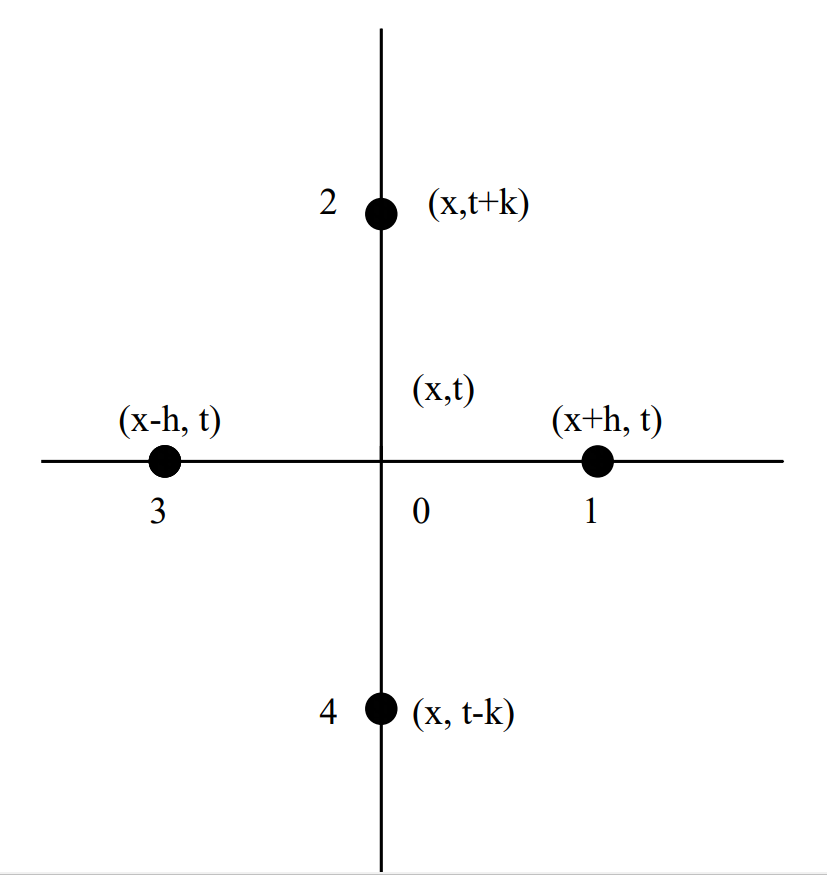
\includegraphics[height = 0.62 \textheight]{img/23/stab1}}
\end{frame}

\begin{frame}
$$u_{xx} = \frac{u(x-h,t)-2u(x,t)+u(x+h,t)}{h^2},$$
$$u_{tt} = \frac{u(x,t+k)-2u(x,t)+u(x,t-k)}{k^2},$$
czyli przybliżeniem (\ref{etykieta}) jest: \\
\begin{equation} \label{21} u(x,t+k) = 2\cdot u(x,t) - u(x,t-k) + \frac{k^2}{h^2}[u(x-h,t)-2u(x,t)+u(x+h,t)] \end{equation}
Dla wyznaczenia $u$ w pierwszym wierszu $\Rightarrow$ przybliżenie (\ref{second}):
$$u_t(x,0) \approx \frac{u(x,k) - u(x,0)}{k} = f_2(x)$$
czyli:
\begin{equation} \label{22} u(x,k) = u(x,0) + k \cdot f_2(x) \end{equation}
\end{frame}

\begin{frame}
  \begin{exampleblock}{Przykład}
      \begin{enumerate}[I.]
       \item $u(x,0) = x \quad 0 \le x \le 1$ \\
	\item $u_t(x,0) = 1\quad 0 < x < 1$ \\
      \item $u(0,t) = 0 \quad t \le 0$ \\
	\item $u(1,t) = 1 \quad t \le 0$
\end{enumerate}
  \end{exampleblock}
\vspace{5mm}
Zobaczymy, co będzie, gdy h = $\frac{1}{6}, k =\frac{1}{2}$ i pominiemy w. b. III) i IV) \\
\vspace{5mm}
z (\ref{22}) i I): $u_1 = \frac{2}{3}, u_2 = \frac{5}{6}, u_3 = 1, u_4 = \frac{7}{6}, u_5 = \frac{4}{3}$ \\
\vspace{3mm}
z (\ref{21}): $u_7 = \frac{4}{3}, u_8 = \frac{3}{2}, u_9 = \frac{5}{3}$
\end{frame}

\begin{frame}
 \centerline{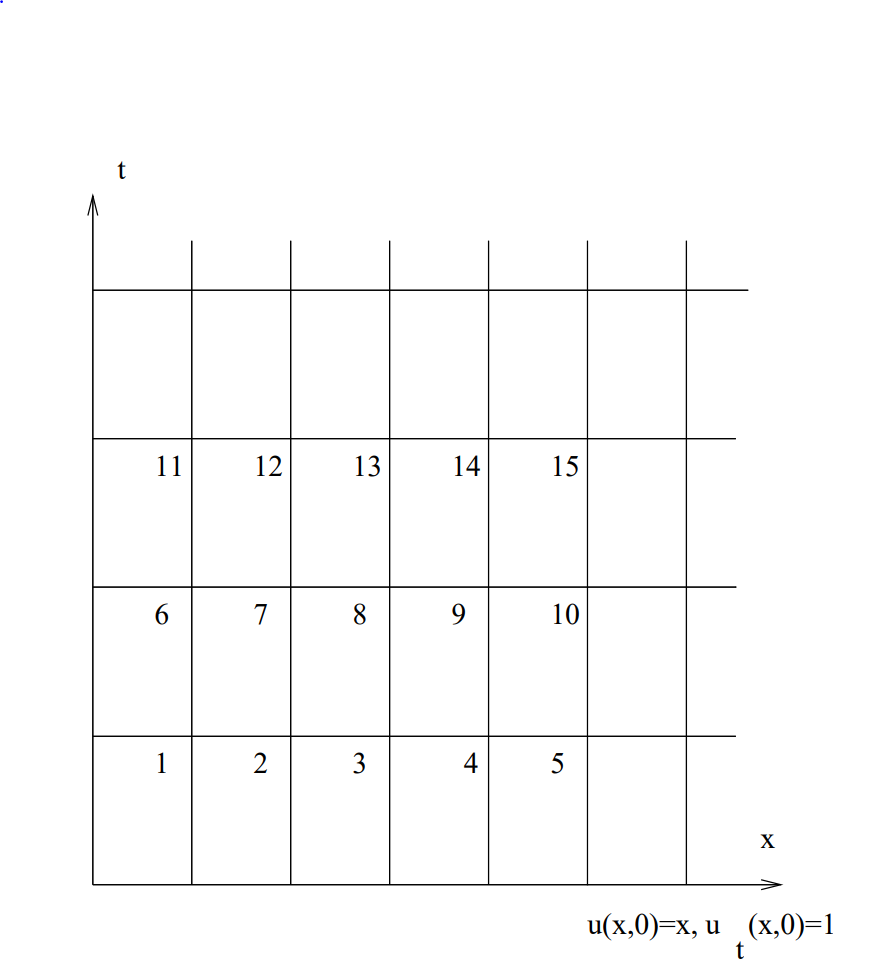
\includegraphics[height = 1 \textheight]{img/23/stab2}}
\end{frame}

\begin{frame}
\begin{alertblock}{Ale...}
\begin{itemize}
  \item  $u_6, u_{10} $ -- nie może być wyznaczone! 	
\item i wreszcie $u_{13} = 2$
 \item przy pominiętych III) i IV) \\
$\Rightarrow u$ tylko w trójkącie $(0,0), (1,0),\underbrace{\left ( \frac{1}{2}, \frac{1}{2} \right )}_{\#3} ! $
\end{itemize}
 \end{alertblock}

\vspace{6mm}
usunięcie niezgodności: $k \le h$ (warunek stabilności dla (\ref{21})) \\
$\Rightarrow$ jest to \textbf{Explicit Method for Initial-Boundary Problems}
\end{frame}


